% compile by  pdflatex blog; biber blog
% GitHub cvitanov/reducesymm/dasgroup/holonomies.tex


\chapter{Exotic symplectic holonomies}
\label{c-holonomies}

%%%%%%%%% Bryant\rf{Bryant99} macros %%%%%%%%%%%%%%%%%%%%%
\def\Lam{\hbox{\sans\char3}}%sans Lambda
\def\Sym{\hbox{\sans S}}
\def\SO{{\rm SO}}\def\SL{{\rm SL}}
\def\Sp{{\rm Sp}}\def\SU{{\rm SU}}
\def\CO{{\rm CO}}\def\GL{{\rm GL}}
\def\Spin{{\rm Spin}}\def\U{{\rm U}}
\def\A{{\rm A}}\def\C{{\rm C}}\def\D{{\rm D}}
\def\E{{\rm E}}\def\O{{\rm O}}
\def\Diff{{\rm Diff}}\def\G{{\rm G}}
\def\bbC{{\Bbb C}}
\def\bbF{{\Bbb F}}
\def\bbH{{\Bbb H}}
% font for Schur functor symbols: CM sans serif
\font\sans=cmss10
%%%%%%%%% Bryant\rf{Bryant99} macros %%%%%%%%%%%%%%%%%%%%%

%%%%%%%%%%%%%%%%%%%% Bryant\rf{Bryant99} Table~IV %%%%%%%%%%%%%%
% reducesymm/dasgroup/Bryant99tabIV.tex
% Predrag  2015-12-03

%%%%%%%%% Bryant\rf{Bryant99} macros %%%%%%%%%%%%%%%%%%%%%
\def\Lam{\hbox{\sans\char3}}%sans Lambda
\def\Sym{\hbox{\sans S}}
\def\SO{{\rm SO}}\def\SL{{\rm SL}}
\def\Sp{{\rm Sp}}\def\SU{{\rm SU}}
\def\CO{{\rm CO}}\def\GL{{\rm GL}}
\def\Spin{{\rm Spin}}\def\U{{\rm U}}
\def\A{{\rm A}}\def\C{{\rm C}}\def\D{{\rm D}}
\def\E{{\rm E}}\def\O{{\rm O}}
\def\Diff{{\rm Diff}}\def\G{{\rm G}}
\def\bbC{{\Bbb C}}
\def\bbF{{\Bbb F}}
\def\bbH{{\Bbb H}}
%definition of the font for footnotes
\font\ninerm=cmr9%
% font for Schur functor symbols: CM sans serif
\font\sans=cmss10
%%%%%%%%% Bryant\rf{Bryant99} macros %%%%%%%%%%%%%%%%%%%%%
\begin{table}
\centerline{
\vtop{
\offinterlineskip
\halign{
&\vrule#&\strut\quad\hfil#\hfil\quad\cr  %The preamble
\multispan4{\hfil \bf IV. Exotic Symplectic Holonomies \hfil}\cr
\noalign{\smallskip}
\multispan4{\hrulefill}&\cr
height 2 pt&\omit&&\omit&\cr
& H && ${\mathfrak m}$ &\cr
height 2 pt&\omit&&\omit&\cr
\multispan4{\hrulefill}&\cr
height 1 pt&\omit&&\omit&\cr
\multispan4{\hrulefill}&\cr
height 2 pt&\omit&&\omit&\cr
&   &&   &\cr
height 3 pt&\omit&&\omit&\cr
\multispan4{\hrulefill}&\cr
height 2 pt&\omit&&\omit&\cr
& $\SL(2,\bbR)$ && $\bbR^4\simeq\Sym^3(\bbR^2)$ &\cr
height 1 pt&\omit&&\omit&\cr
& $\SL(2,\bbC)$ && $\bbC^4\simeq\Sym^3(\bbC^2)$ &\cr
height 2 pt&\omit&&\omit&\cr
\multispan4{\hrulefill}&\cr
height 2 pt&\omit&&\omit&\cr
& $\SL(2,\bbR)\!\cdot\!\SO(p,q)\,^a$ && $\bbR^{2}\otimes\bbR^{p+q}$ &\cr
height 1 pt&\omit&&\omit&\cr
& $\SL(2,\bbC)\!\cdot\!\SO(n,\bbC)\,^b$ && $\bbC^{2}\otimes\bbC^{n}$ &\cr
height 1 pt&\omit&&\omit&\cr
& $\Sp(1)\!\cdot\!\SO(n,\bbH)\,^c$ && $\bbH^{n}$ &\cr
height 2 pt&\omit&&\omit&\cr
\multispan4{\hrulefill}&\cr
height 2 pt&\omit&&\omit&\cr
& $\Sp(3,\bbR)$ && $\bbR^{14}\simeq \Lam^3_0(\bbR^6)$ &\cr
height 1 pt&\omit&&\omit&\cr
& $\Sp(3,\bbC)$ && $\bbC^{14}\simeq \Lam^3_0(\bbC^6)$ &\cr
height 2 pt&\omit&&\omit&\cr
\multispan4{\hrulefill}&\cr
height 2 pt&\omit&&\omit&\cr
& $\SL(6,\bbR)$ && $\bbR^{20}\simeq\Lam^3(\bbR^6)\phantom{^\bbR}$ &\cr
height 1 pt&\omit&&\omit&\cr
& $\SU(1,5)$ && $\bbR^{20}\simeq\Lam^3(\bbC^6)^\bbR$ &\cr
height 1 pt&\omit&&\omit&\cr
& $\SU(3,3)$ && $\bbR^{20}\simeq\Lam^3(\bbC^6)^\bbR$ &\cr
height 1 pt&\omit&&\omit&\cr
& $\SL(6,\bbC)$ && $\bbC^{20}\simeq\Lam^3(\bbC^6)\phantom{^\bbR}$ &\cr
height 2 pt&\omit&&\omit&\cr
\multispan4{\hrulefill}&\cr
height 2 pt&\omit&&\omit&\cr
& $\Spin(2,10)$ && $\bbR^{32}$ &\cr
height 1 pt&\omit&&\omit&\cr
& $\Spin(6,6)$ && $\bbR^{32}$ &\cr
height 1 pt&\omit&&\omit&\cr
& $\Spin(6,\bbH)$ && $\bbR^{32}$ &\cr
height 1 pt&\omit&&\omit&\cr
& $\Spin(12,\bbC)$ && $\bbC^{32}$ &\cr
height 2 pt&\omit&&\omit&\cr
\multispan4{\hrulefill}&\cr
height 2 pt&\omit&&\omit&\cr
& $\E_7^5$ && $\bbR^{56}$ &\cr
height 1 pt&\omit&&\omit&\cr
& $\E_7^7$ && $\bbR^{56}$ &\cr
height 1 pt&\omit&&\omit&\cr
& $\E_7^\bbC$ && $\bbC^{56}$ &\cr
height 2 pt&\omit&&\omit&\cr
\multispan4{\hrulefill}&\cr
}
}
%\vskip-10pt}
\hskip1pt
\vtop{\offinterlineskip
\halign{
&\vrule#&\strut\quad\hfil#\hfil\quad\cr  %The preamble
\multispan4{\hfil \bf $\E_7$ row \hfil}\cr
\noalign{\smallskip}
\multispan4{\hrulefill}&\cr
height 2 pt&\omit&&\omit&\cr
& algebra && rep. &\cr
height 2 pt&\omit&&\omit&\cr
\multispan4{\hrulefill}&\cr
height 1 pt&\omit&&\omit&\cr
\multispan4{\hrulefill}&\cr
height 2 pt&\omit&&\omit&\cr
& $\U(1)  $ && $\bbR^{2}$ &\cr
height 3 pt&\omit&&\omit&\cr
\multispan4{\hrulefill}&\cr
height 2 pt&\omit&&\omit&\cr
& $\A_1  $ && $\bbR^{4}$ &\cr
height 1 pt&\omit&&\omit&\cr
&   &&   &\cr
height 3 pt&\omit&&\omit&\cr
\multispan4{\hrulefill}&\cr
height 2 pt&\omit&&\omit&\cr
& $3\,\A_1$ && $\bbR^{8}$ &\cr
height 1 pt&\omit&&\omit&\cr
&   &&   &\cr
height 1 pt&\omit&&\omit&\cr
&   &&   &\cr
height 3 pt&\omit&&\omit&\cr
\multispan4{\hrulefill}&\cr
height 2 pt&\omit&&\omit&\cr
& $\C_3$ && $\bbR^{14}$ &\cr
height 1 pt&\omit&&\omit&\cr
&   &&   &\cr
height 3 pt&\omit&&\omit&\cr
\multispan4{\hrulefill}&\cr
height 2 pt&\omit&&\omit&\cr
& $\A_5  $ && $\bbR^{20}$ &\cr
height 1 pt&\omit&&\omit&\cr
&   &&   &\cr
height 1 pt&\omit&&\omit&\cr
&   &&   &\cr
height 1 pt&\omit&&\omit&\cr
&   &&   &\cr
height 3 pt&\omit&&\omit&\cr
\multispan4{\hrulefill}&\cr
height 2 pt&\omit&&\omit&\cr
& $\D_6  $ && $\bbR^{32}$ &\cr
height 1 pt&\omit&&\omit&\cr
&   &&   &\cr
height 1 pt&\omit&&\omit&\cr
&   &&   &\cr
height 1 pt&\omit&&\omit&\cr
&   &&   &\cr
height 3 pt&\omit&&\omit&\cr
\multispan4{\hrulefill}&\cr
height 2 pt&\omit&&\omit&\cr
& $\E_7  $ && $\bbR^{56}$ &\cr
height 1 pt&\omit&&\omit&\cr
&   &&   &\cr
height 1 pt&\omit&&\omit&\cr
&   &&   &\cr
height 3 pt&\omit&&\omit&\cr
\multispan4{\hrulefill}&\cr
}
%\vskip-10pt
}
}
\caption{\label{Bryant99tabIV}
(left)
Bryant Table~IV\rf{Bryant99}.
The $H$ are subgroups of~$\Sp(S)\subset\GL({\mathfrak m})$ for a
nondegenerate skew symmetric bilinear form~$S$ on~${\mathfrak m}$, and the
corresponding $H$-structures have an underlying symplectic structure.
The restrictions are
$(a)$ {\ninerm $p+q\ge3$} (for irreducibility),
$(b)$ {\ninerm $n\ge3$} (for irreducibility),
and
$(c)$ {\ninerm $n\ge2$} (to be nonmetric).
(right)
The $\E_7$ row\rf{NegDimE7} of the Magic Triangle\rf{PCar,C77,PCgr}.
}
\end{table}
%%%%%%%%%%%%%%%%%%%%%%%%%%%%%%%%%%%%%%%%%%%%%%%%%%%%%%%%%%%%%%%%%%%%%%%

%%%%%%%%%%%%%%%%%%%% Bryant\rf{Bryant99} Table~IV %%%%%%%%%%%%%%

On 2016-10-24 Bernard Julia wrote to Predrag:
\begin{quote}
I recently found a niche for your $E_7$ family\rf{NegDimE7}. Please have a
look at Bryant\rf{Bryant99} and check out \reftab{Bryant99tabIV} in his
review of Berger\rf{Berger55,Berger57} nonmetric holonomies.
You will find among the exotic symplectics \(E_7, D_6, A_5\) (where everybody
agrees), and then your $C_3$, your $3\,A_1$ (as a possible solution) and your
$A_1$.

What do you make of this, except that the symplecticity is just right... ?

I copy this to Pierre <pierre.ramond@gmail.com> who may appreciate.
\end{quote}

\bigskip

My 1975 construction\rf{PCar,C77,PCgr} of the $\E_7$ row of the Magic
Triangle was inspired by Brown's\rf{Brown1969} observation that defining
representation of \(E_7\) has a symmetric quartic invariant (my construction,
however, is a stand-alone derivation that owes nothing to Brown and
Freudethal). In my {\em Negative dimensions and $E_7$
symmetry}\rf{NegDimE7} (as well as in Chapter 20. {\em $E_7$ family and its
negative-dimensional cousins} of the birdtracks book\rf{PCgr}) I the
negative-dimension relation through which $E_7$ emerges as a
negative-dimensional relative of $SO(4)$.
As nobody understood my diagrammatic notation, in 1980 I rewrote my (very
compact in diagrammatic notation) derivation of the $\E_7$ family in the more
standard and lengthy index notation\rf{NegDimE7}. That also ended up
blowing in the wind.

\medskip

My reading Bryant\rf{Bryant99} review paper
{\em Recent advances in the theory of holonomy},
\\ \arXiv{math/9910059}
\\~[arXiv now includes blog links:
\HREF{https://en.wikipedia.org/wiki/Holonomy}{wiki/Holonomy}
and
\HREF{http://mathoverflow.net/questions/6475/what-is-the-relationship-between-various-things-called-holonomic/6550\#6550}
{mathoverflow}]:


{\it Exotic Holonomies.}
The full list of exotic holonomies (so called because the were omitted from
the initial list of Berger\rf{Berger57}) was compiled by Chi, Merkulov,
Schwachh\"ofer, and Bryant\rf{ChMeSc96,Bryant87,Bryant91}; see, in
particular, the tables in Merkulov and
Schwachh{\"o}fer\rf{MerSch99,MerSch99add}, and \reftab{Bryant99tabIV} here.

The first two examples in \reftab{Bryant99tabIV}, each with a torsion-free
connection, were analyzed in \refref{Berger57}. The
study\rf{Bryant87,Bryant91} of the moduli space of rational curves on a
complex surface with normal bundle~${\cal O}(3)$ turned up the next two
entries in \reftab{Bryant99tabIV} that were omitted from Berger's nonmetric
list\rf{Bryant91}. The `exotic' refers to any nonmetric
subgroup~$H\subset\GL({\mathfrak m})$ that satisfies Berger's criteria but
that does not appear on Berger's original nonmetric list.
The construction \rf{Bryant91} uncovered a number of unexpected identities.
Chi, Merkulov, and Schwachh\"ofer\rf{ChMeSc96} found other exotic symplectic
examples, and noticed that the reconstruction technique generalized in the
context of Poisson geometry (\ie, Poisson bracket, or a symplectic
skew-symmetric invariant).

% Even for the exceptional holonomies, there are explicit examples of
% cohomogeneity one\rf{Bryant87,BrySal89}.

\bigskip

I am not able to decode any of the ``exotic holonomies'' literature that I
have looked at. Questions to experts:

\begin{description}
  \item[(quartic invariant)]
Is there is a quartic invariant someplace in the Poisson manifolds derivation
of the exotic symplectic holonomies?
  \item[(ternary algebra)]
If not that, can you identify a class of ternary algebras (Freudenthal triple
systems), see Faulkner\rf{Faulkner1971} and Yamaguti and
Asano\rf{Yamaguti1975}.
  \item[($3\,A_1$)]
Is my 8-dimensional representation of semi-simple $3\,A_1$ consistent with your
family of possible symmetries? I have no wiggle room - it must be $\bbR^{8}$.
Would there be something special about that case?
  \item[($\U(1)$)]
Why don't you have $\U(1)  $, $\bbR^{2}$ in your list?
Too trivial for you?
  \item[(supersymmetry)]
Where is the list of supersymmetric partners\rf{MerSch99} to
\reftab{Bryant99tabIV}?
Is
\(\SOn{4} \simeq \SOn{3}\oplus\SOn{3} \simeq A_1\oplus A_1
\)
in such list?
  \item[(exceptional magic)] Would it make you happy to learn that
your `exotic' is a synonym for Cartan-Kylling's `exceptional'\rf{PCgr}?

\end{description}

\section{Holonomies blog}
\label{s-HolonomBlog}

\begin{description}

\item[2016-12-03 Predrag]
Merkulov and Schwachh{\"o}fer\rf{MerSch99} note
``
Another by-product result is  the striking supersymmetry property of their
real forms which occur as holonomies of torsion-free affine connections. With
any symplectic Lie algebra $g \subset \Sp(V)$, dim~$g = m$, dim~$V = 2n$, one
may associate naturally an $(m|2n)$-dimensional supermanifold
''

Supersymmetry was actually the motivation for construction of my my $\E_7$
family\rf{NegDimE7}, but I have so far not been able to identify my $\SOn{4}$
family in the above holonomies literature. It might be in this
paper\rf{MerSch99}, for all I know...

\item[2016-12-03 Predrag]
\HREF{https://math.duke.edu/people/robert-bryant} {Robert Bryant}
% <bryant@math.duke.edu>, Duke University.
is not only the current President of the American Mathematical Society.
American Mathematical Society, he is also a NAS, and Landsberg's thesis
adviser, etc. He explains the idea of ``holonomy'' by a
\HREF{http://www.maa.org/meetings/calendar-events/the-idea-of-holonomy}
{basketball}.

\item[2016-12-07 Robert Bryant]

I haven't been thinking about these things for a very long time, so your
questions probably would be better going to Chi, Merkulov, and/or
Schwachhofer.  I'll tell you what I know about your questions, but it's not
much:

Quartic invariant:
There are quartic polynomial invariants associated to these things in all cases.

        For example, $\Spin(2,10)$ (up to a finite extension) acting on $\bbR^{32}$
        is defined as the stabilizer of a certain quartic polynomial in 32
        variables, and, of course, it also stabilizes a symplectic form on
        $\bbR^{32}$.  Similarly $E_7$ (up to a finite extension) acting on $\bbR^{56}$ is
        defined by the quartic polynomial originally defined by Cartan.

        The lower dimensions are classical:

For $A_1$ acting on $\bbR^4 =
        S^3(\bbR^2)$, which is the homogeneous cubics in two variables, the
        quartic is the classical discriminant of a cubic form in two
        variables.

For $3\,A_1$ acting on $\bbR^8 = \bbR^2\otimes \bbR^2 \otimes \bbR^2$, the
        quartic invariant was discovered by Cayley in 1843 and is known as
        Cayley's hyperdeterminant.

In the case of $A_5$ acting on $\bbR^{20} =
        \Lambda^3(\bbR^6)$, there is a well-known quartic invariant polynomial,
        and $A_5$ is the stabilizer of that polynomial.

The $C_3$ case turns out
        to be the restriction of that quartic polynomial to the
        14-dimensional invariant subspace of $\bbR^{20}$ that $C_3$ preserves.

        You can find details on this material by searching for the term
        'prehomogeneous vector spaces' in the literature.

Ternary algebra:  I know nothing about this.

$3\,A_1$ :  I don't know of anything particularly special about this that makes it
somehow nicer than the other cases.  I'm not sure what your 'wriggle room'
means.  There are other real forms, besides the Cayley hyperdeterminant case
(which is the natural choice for 'split form'); there are 4 distinct real
forms altogether in the (real) 8-dimensional case.

$U(1)$:  Yes, this case is 'trivial' because it actually preserves a quadratic
form (whose square is, of course, the invariant quartic form), and so it has
already been accounted for in the metric case.

Supersymmetry:  I don't know anything about this.

Exceptional Magic:  I think 'synonym' is too strong a word, here.  Clearly,
there is a connection of the exotic symplectic holonomies with the
exceptional groups, but it's not one-to-one.  You can find more about this in
the 'Affine Holonomy' section (near the end) of the Wikipedia page
https://en.wikipedia.org/wiki/Holonomy.  There is also a paper by Cahen and
Schwachh{\"o}fer\rf{CahSch99} in which they discuss this at length and its
relation with Poisson structures.

        That's all that I know.

        Yours,

        Robert Bryant

\item[2016-12-08 Predrag] Recheck

Wybourne\rf{Wybourne78}
{\em {$SU_6 \times SU_{3c}$} scalars in $E_7$ irreps}

Butler, Haase and Wybourne\rf{Butler1978}
{\em Calculation of {$3jm$} factors and the matrix elements of {$E_7$} group generators}

Butler, Haase and Wybourne\rf{Butler78a}
{\em Calculation of {$6j$} symbols for the exceptional group {$E_7$}}

Wybourne\rf{Wybourne80}
{\em Enumeration of group invariant quartic polynomials in {Higgs} scalar fields}

\begin{figure}% [H]
  \begin{center}
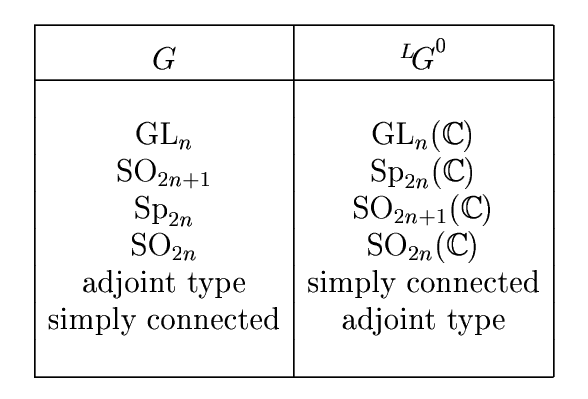
\includegraphics[width=0.55\textwidth]{Langlands}
  \end{center}
\caption{
Langlands duality (Simon Burton).
}
\label{fig:Langlands}
\end{figure}


\item[2021-07-20 Simon Burton]
\HREF{https://twitter.com/fridaysimon/status/1417463478755942403}
{@fridaysimon}
\\
I wonder if these
\HREF{http://birdtracks.eu/version9.0/GroupTheory.pdf\#chapter.13}
{"negative dimension" Lie groups} from the {birdtracks book} correspond
to Langlands dual groups.

\item[2021-07-20 John Carlos Baez]
\HREF{https://twitter.com/johncarlosbaez/status/1417504419579535363}
{@johncarlosbaez}
\\
Interesting.  I don't think so: the birdtracks book switches Sp(2n) and
SO(2n), while Langlands duality switches Sp(2n) and SO(2n+1).   The
Dynkin diagrams of Sp(2n) and SO(2n+1) are almost the same, and identical
when n is 1 or 2.

There's a way in which is Sp(2n) is very much like SO(2n): one preserves
a skew-symmetric nondegenerate form, the other a symmetric one.  And
there's a subtler way in which Sp(2n) is like SO(2n+1), visible from
their Dynkin diagrams.

\item[2021-07-24 Predrag]
While I have @fridaysimon @johncarlosbaez attention - glance at
\reftab{Bryant99tabIV} list of
\HREF{https://twitter.com/chaaosbook/status/1418983522748882944} {exotic
holonomies} The same as the $E_7$ row of my Magic Triangle. Robert Bryant
gave me thoughtful, detailed answers (see
\HREF{http://chaosbook.org/~predrag/old/exceptHolo.pdf} {my notes}) but I
do not understand why these families come out the same.








\end{description}
\renewcommand{\ssp}{a}


%\newpage %%%%%%%%%%%%%%%%%%%%%%%%%%%%%%%%%%%%%%%%%%%%%%%%
\printbibliography[heading=subbibintoc,title={References}]
